\documentclass[11pt]{article}
\usepackage[spanish]{babel}
\usepackage{natbib}
\usepackage{url}
\usepackage[utf8x]{inputenc}
\usepackage{amsmath}
\usepackage{amssymb}
\usepackage{graphicx}
\graphicspath{{images/}}
\usepackage{parskip}
\usepackage{fancyhdr}
\usepackage{vmargin}
\usepackage{natbib}
\usepackage{apalike}

\setmarginsrb{3 cm}{2.5 cm}{3 cm}{2.5 cm}{1 cm}{1.5 cm}{1 cm}{1.5 cm}

\title{Proyectos}						% Title
\author{J. Eduardo Sánchez Posadas}					%Author
\date{\today}											% Date

\makeatletter
\let\thetitle\@title
\let\theauthor\@author
\let\thedate\@date
\makeatother

\pagestyle{fancy}
\fancyhf{}
\rhead{GUI con Java}
\lhead{\thetitle}
\rfoot{\thepage}
\lfoot{FES Aragón - UNAM}

\begin{document}

%%%%%%%%%%%%%%%%%%%%%%%%%%%%%%%%%%%%%%%%%%%%%%%%%%%%%%%%%%%%%%%%%%%%%%%%%%%%%%%%%%%%%%%%%

\begin{titlepage}
	\centering
    \vspace*{0.5 cm}
    \includegraphics[scale=0.05]{pics/escudo.png} \\[1.0 cm]	% University Logo
    \textsc{\Huge Universidad Nacional Autónoma de México}\\[2.0 cm]	% University Name
	\textsc{\Huge FES Aragón\\ Ingeniería en Computación}\\[0.5 cm]								% Course Code
	\textsc{\Large Interfaces Gráficas de Usuario \\ con Java}\\[0.5 cm]	% Course Name
	\rule{\linewidth}{0.2 mm} \\[0.4 cm]
	{ \huge \bfseries \thetitle}\\
	\rule{\linewidth}{0.2 mm} \\[1.5 cm]
	 			{Autor: \large \theauthor}
% 	\begin{minipage}{0.4\textwidth}
% 		\begin{flushleft} \large
% 			\emph{Nombre: Nombre(s) Apellido(s]}\\
%
% 			\end{flushleft}
% 			\end{minipage}~
% 			\begin{minipage}{0.4\textwidth}
% 			\begin{flushright} \large
% 			\emph{Número de Cuenta} \\
% 											% Your Student Number
% 		\end{flushright}
% 	\end{minipage}\\[2 cm]
	
	{\large \thedate}\\[2 cm]
 
	\vfill
	
\end{titlepage}

%%%%%%%%%%%%%%%%%%%%%%%%%%%%%%%%%%%%%%%%%%%%%%%%%%%%%%%%%%%%%%%%%%%%%%%%%%%%%%%%%%%%%%%%%

\tableofcontents
\pagebreak

%%%%%%%%%%%%%%%%%%%%%%%%%%%%%%%%%%%%%%%%%%%%%%%%%%%%%%%%%%%%%%%%%%%%%%%%%%%%%%%%%%%%%%%%%

\section{Generador de Funciones Senoidales}
\subsection{Introducción}

Un \emph{generador de señales}, de \emph{funciones} o de \emph{formas de onda} es un dispositivo electrónico de laboratorio que genera patrones de señales periódicas o no periódicas tanto analógicas como digitales. Se emplea normalmente en el diseño, prueba y reparación de dispositivos electrónicos; aunque también puede tener usos artísticos.

Hay diferentes tipos de generadores de señales según el propósito y aplicación que corresponderá con el precio. Tradicionalmente los generadores de señales eran dispositivos estáticos apenas configurables, pero actualmente permiten la conexión y control desde un PC. Con lo que pueden ser controlados mediante software hecho a medida según la aplicación, aumentando la flexibilidad. \citep{gdf}

\subsection{Señal}
\textbf{Señal}: se define como una magnitud física o detectable mediante la que se puede transmitir mensajes o información. Matemáticamente una señal es una función de una variable independiente. Ejemplo: 
$$x(t) = 3\sin(2t)$$
En el ejemplo anterior $t$ es la variable independiente.
Ejemplos en la realidad:
\begin{itemize}
\item Señales de audio de micrófono
\item Voltaje o intensidad en un circuito
\item Flujo de bits en proporcionados por un ordenador \citep{iss}
\end{itemize}

\begin{figure}[h]
\centering
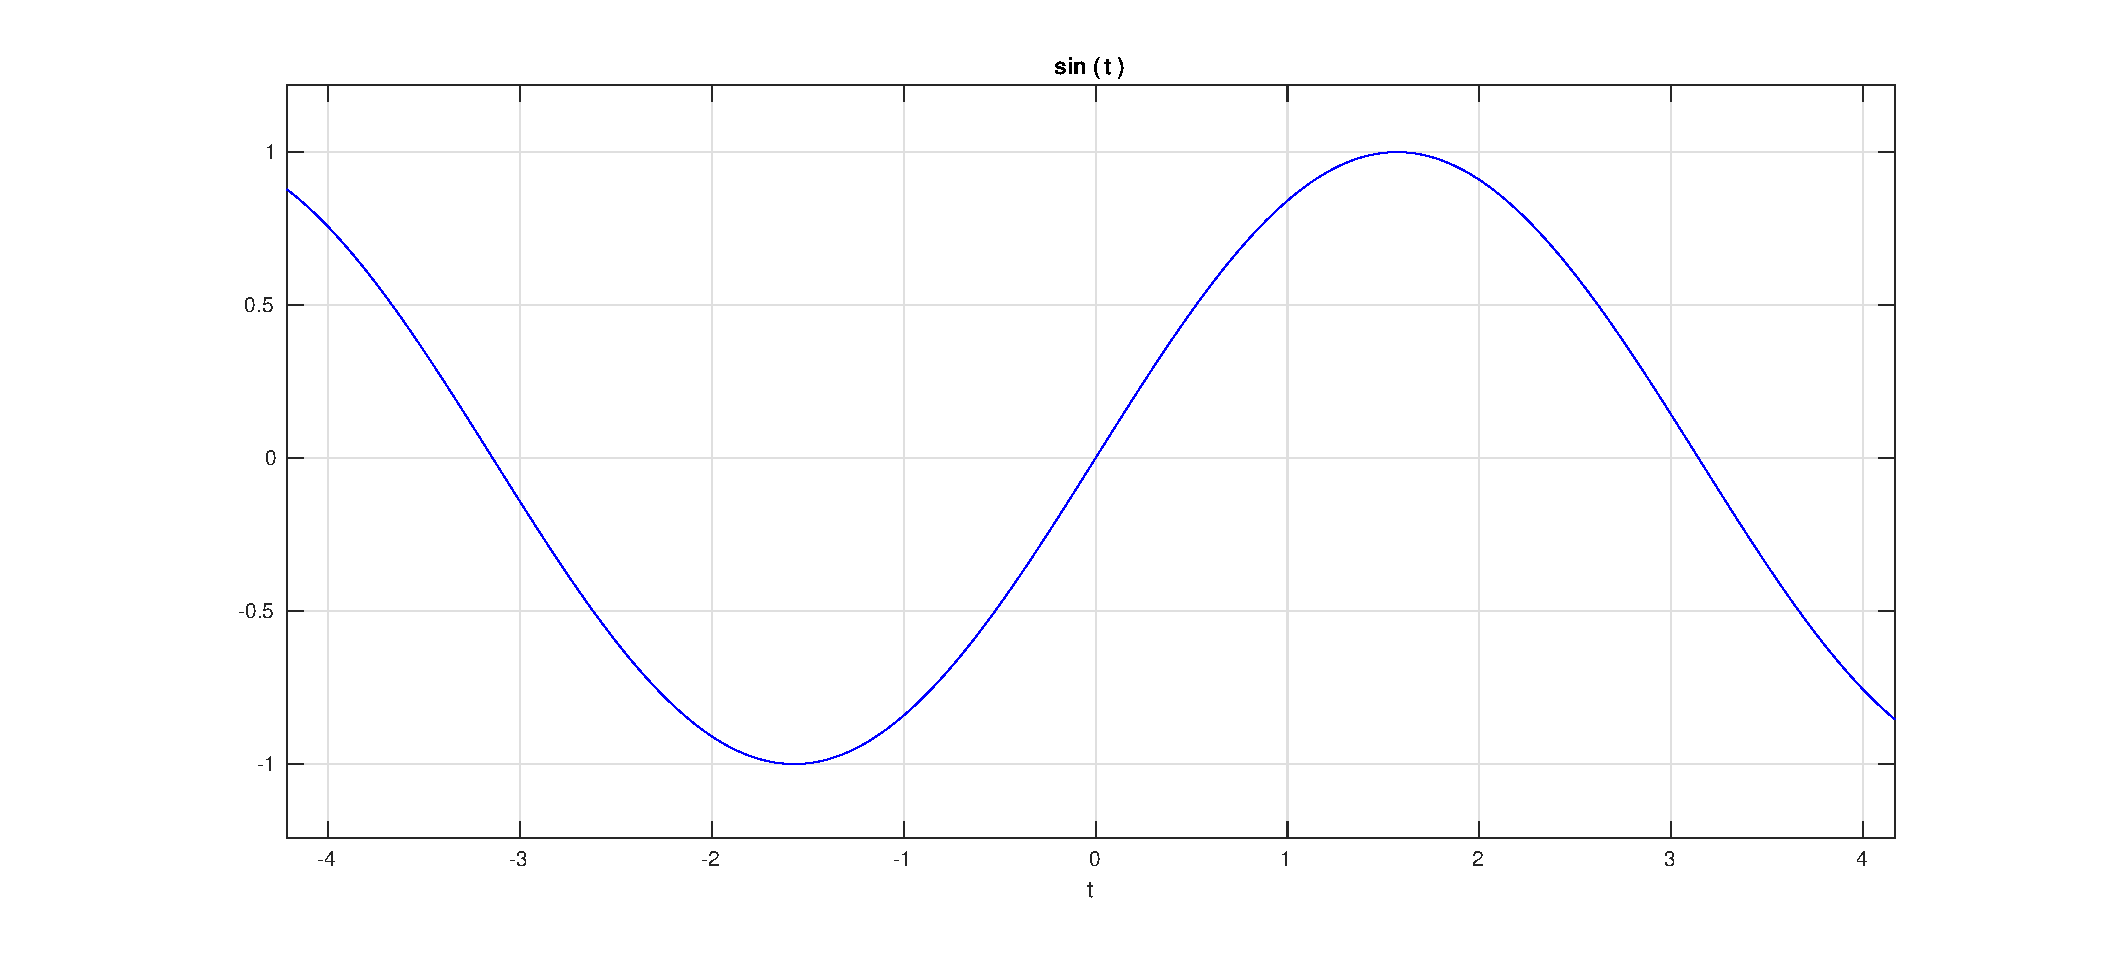
\includegraphics[scale=0.3]{pics/sin.eps} 
\caption{Señal $y(t) = \sin(t)$}
\end{figure}
\newpage
Una señal senoidal puede ser descrita por las siguientes expresiones matamáticas: 

$$y(x)=A \sin(\omega x + \phi)$$
$$y(x)=A \sin(2\pi ft + \phi)$$
$$y(x)=A \sin \left(\frac{2\pi}{T}x+\phi\right)$$
donde:\\
\begin{itemize}
\item $A$ es la apmlitud de oscilación.
\item $\omega$ es la velocidad angular; $\omega=2\pi f$
\item $f$ es la frecuencia de oscilación.
\item $T$ es el periodo de oscilación; $T=1/f$
\item $\omega x + \phi$ es la fase de oscilación.
\item $\phi$ es la fase inicial.
\end{itemize}

\begin{figure}
\centering
\includegraphics[scale=0.7]{pics/sin_c.png} 
\caption{Caracteristicas de una señal senoidal}
\end{figure}

\subsection{Requerimientos}
Debe realizar una aplicación en Java con interfáz gráfica donde se pueda graficar señales senoidal y cosenoidal. Debe tener mínimo lo siguiente:

\begin{itemize}
\item Elegir entre senoidal y cosenoidal
\item Modificar amplitud
\item Modificar frecuencia
\item Modificar el \emph{offset}\footnote{Es el desplzazamiento vertical de la señal}
\item Modificar la fase de oscilación
\item Añadir mas de una señal
\item Modificar el color de la señal
\item Mostrar valor pico-pico
\item Mostrar valor RMS de la señal
\item Guardar una imagen en JPEG o PNG
\item Malla
\end{itemize}

A continuación se sugiere la interfáz gráfica:


\begin{figure}
\centering
\includegraphics[scale=0.5]{pics/pic3.png}
\caption{Sugerencia de interfáz gráfica para este proyecto.}
\end{figure}




\newpage
\bibliographystyle{apalike}

\section{Sistema de Votacion}


\bibliography{biblist}

\end{document}
